\subsection{Experimental Setup and Hyperparameters} For all experiments, we use Qwen2.5-7B-Instruct without quantization. To ensure fair comparison, all experiments use the same seed, temperature, and status prompt. Specifically, we set the seed equal to the episode number, since a fixed seed would result in the environment always being the same, and temperature to 0 to ensure determinism. All experiments calculate the average metrics across 20 episodes, with a maximum allowed steps of 100 per episode and no limit on the number of tokens the agent may use. 

All prompting strategies are compared to the baseline that simply asks for the model to predict an action. The first evaluation metric is the Success Rate (SR), which measures how often the agent reaches the goal in the environment. To quantify efficiency, we also measure the average steps taken to reach the goal and the average tokens (input and output) used to take an action. Finally, we quantify the cost efficiency using the average steps taken to reach the goal. 

\subsection{Experimental Result}

\tableautorefname~ \ref{tab:empty8x8} shows our results on the Empty8x8 environment, \tableautorefname~ \ref{tab:lavagap} the results on LavaGapS6, and finally \tableautorefname~ \ref{tab:lavacrossing} the results on LavaCrossingS9N2.

\begin{table}[h!]
\centering
\caption{Performance comparison on MiniGrid-Empty-8x8-v0 (Qwen2.5-7B-Instruct)}
\label{tab:empty8x8}
\begin{tabular}{lcccc}
\toprule
Method & Success Rate (SR) & Steps & Tokens per Step & Tokens per Rollout\\
\midrule
Baseline           & 100.00\% & 11.60 & 192.57 & 2233.81\\
ReAct              &  90.00\% & 46.33 & 378.52 & 17536.83\\
Chain of Thought   & 100.00\% & 16.60 & 617.50 & 10250.5\\
Tree of Thought    & 100.00\% & 11.00 & 2817.58 & 30993.38\\
Buffer of Thought  & 100.00\% & 11.00 & 207.45 & 2281.95\\
\bottomrule
\end{tabular}
\end{table}

\begin{table}[h!]
\centering
\caption{Performance comparison on MiniGrid-LavaGapS6-v0 (Qwen2.5-7B-Instruct)}
\label{tab:lavagap}
\begin{tabular}{lcccc}
\toprule
Method & Success Rate (SR) & Steps & Tokens per Step & Tokens per Rollout\\
\midrule
Baseline           & 40.00\% & 21.62 & 206.47 & 4463.88\\
ReAct              & 35.00\% & 23.57 & 400.21 & 9432.95\\
Chain of Thought   & 45.00\% & 15.78 & 670.30 & 10577.33\\
Tree of Thought    & 50.00\% & 10.33 & 2200.56 & 22731.78\\
Buffer of Thought  & 55.00\% & 49.15 & 229.32 & 11271.08\\
\bottomrule
\end{tabular}
\end{table}

\begin{table}[h!]
\centering
\caption{Performance comparison on MiniGrid-LavaCrossingS9N2-v0 (Qwen2.5-7B-Instruct)}
\label{tab:lavacrossing}
\begin{tabular}{lcccc}
\toprule
Method & Success Rate (SR) & Steps & Tokens per Step & Tokens per Rollout\\
\midrule
Baseline           &  5.00\% & 35.00  & 249.11 & 8718.85\\
ReAct              &  0.00\% & ---    & 458.34 & ---\\
Chain of Thought   & 15.00\% & 41.67  & 666.30 & 27764.72\\
Tree of Thought    & 20.00\% & 30.67  & 3466.50 & 106317.56\\
Buffer of Thought  & 10.00\% & 91.30  & 274.6 & 25070.98\\
\bottomrule
\end{tabular}
\end{table}

Nearly all agents achieve a perfect success rate on the easiest environment, Empty8x8. For LavaGapS6, on the other hand, success rates hover around 40-55\%, and on the hardest environment, LavaCrossingS9N2, even the best method achieves only a 20\% success rate. The difficulty of this final environment is due to various factors. The abundance of lava compared to LavaGapS6 increases the number of opportunities for the agent to walk in to lava. The larger grid also makes it so that the agent cannot locate the goal as easily, requiring more exploration. 

Overall, it can be found that the reasoning-enhanced LLM agents outperform the baseline Reactive agent with higher success rate and less exploration steps. \textbf{However, it should be noted that the performance of the ReAct agent is slightly worse than the Reactive one both on success rate and exploration steps.} This might be due to the limited capabilities of a 7B model. When trying to predict thought and action at the same time, it worsens the performance as compared to predicting just the action, as the model now has much more to get right at the same time for a less expressive model within just a single reasoning step as opposed to Chain-of-Thought. We hypothesize that using a bigger model would improve ReAct's performance as compared to the Reactive baseline.

On the other hand, Tree of Thought and Buffer of Thought achieve the best performance overall across the three environments, but with performance tradeoffs. Tree of Thought uses far more tokens than the other methods, while Buffer of Thought takes many more steps, due to its exploratory approach. This underlines the fact that the methods all present the user with a tradeoff, where more sophisticated methods can give better results but at the cost of reduced efficiency. 
Notably, the simple baseline method consistently uses the least tokens compared to any other method. This makes it the most efficient option in terms of tokens, but at the expense of performance.
Fig. \ref{fig:pareto} shows which methods are Pareto-optimal for each environment, with baseline and Buffer of Thought being the only two that are optimal in all environments, meaning that regardless of environment, no other method is objectively superior to these in both success rate and token efficiency.

\begin{figure}[h!]
\centering
\begin{subfigure}[b]{0.48\textwidth}
    \centering
    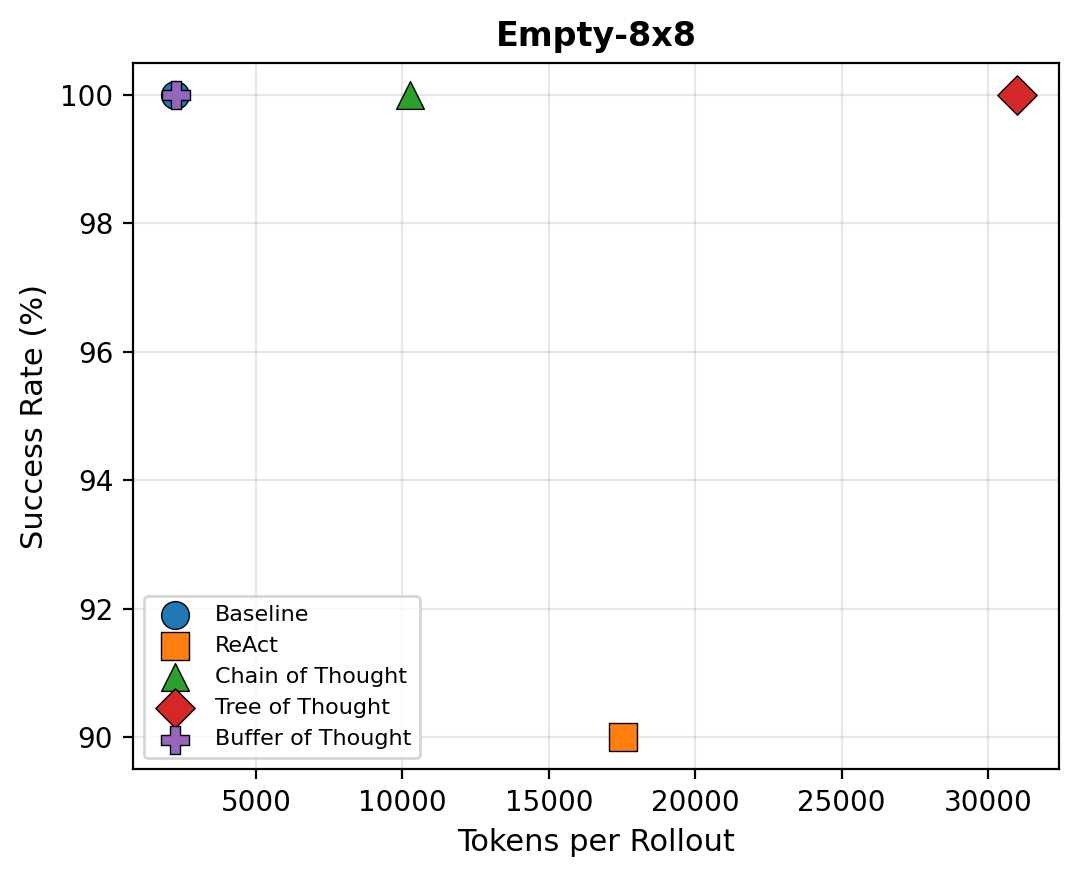
\includegraphics[width=\textwidth]{Figures/pareto_empty8x8.png}
    \label{fig:pareto_empty}
\end{subfigure}
\hfill
\begin{subfigure}[b]{0.48\textwidth}
    \centering
    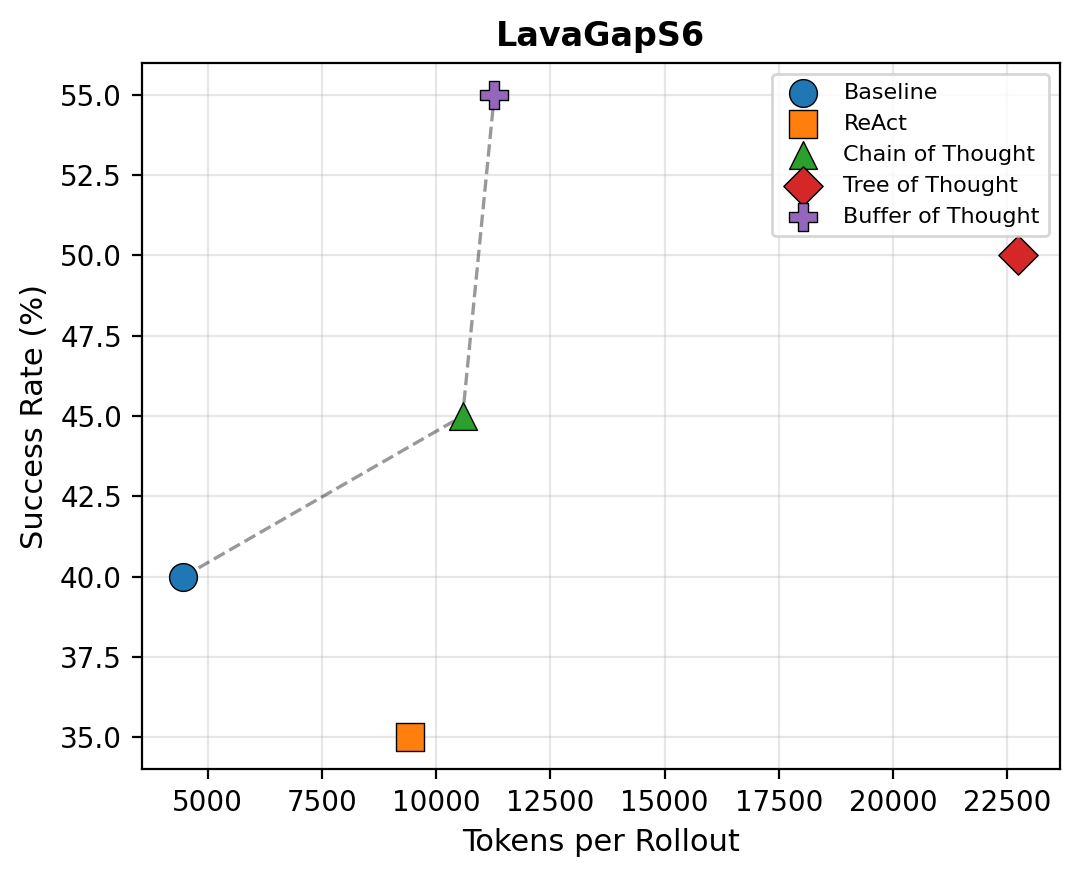
\includegraphics[width=\textwidth]{Figures/pareto_lavagap.png}
    \label{fig:pareto_lavagap}
\end{subfigure}

\vspace{0.5em}

\begin{subfigure}[b]{0.48\textwidth}
    \centering
    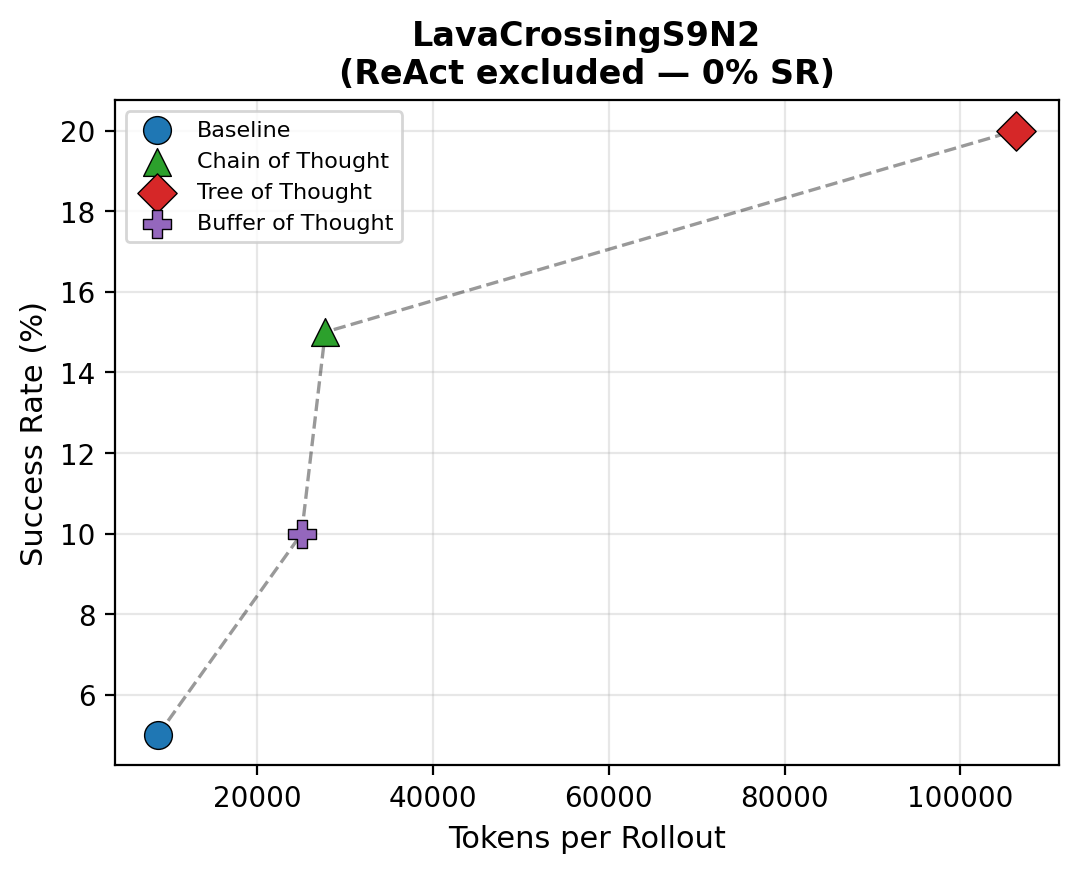
\includegraphics[width=\textwidth]{Figures/pareto_lavacrossing.png}
    \label{fig:pareto_lavacrossing}
\end{subfigure}
\caption{Pareto frontier of success rate vs.\ token cost per rollout across three MiniGrid environments using Qwen2.5-7B-Instruct. The dashed line connects Pareto-optimal methods.}
\label{fig:pareto}
\end{figure}

